\textbf{i. Stochastic gradient descent:}\\
We get features from the first 5 alphabets of first name and last name. As mentioned, '1' is added for each feature to represent $\theta$. To fit line, $\vec{w}\vec{x_i}+\theta = y_i$, to the dataset, we use gradient descent method. Assuming the error function $Q(w)$, we could derive the learning method.
\begin{equation*}
	Q(w) = \frac{1}{2}\sum(\vec{w}\vec{x_i}+\theta - y_i)^2
\end{equation*} 
According to the function, $Q(w)$, we modify the weight vector to minimize error function.
\begin{equation*}
	\vec{w'} = \vec{w} - \eta\times \vec{x_i}(\vec{w}\vec{x_i}+\theta - y_i)
\end{equation*}
Keep adjusting the weight vector until error rate of all training set achieving the threshold we set. Then, we sweep different values for threshold and learning rate. The result:
\begin{center}
\begin{tabular}{|c|c|c|c|c|c|}
\hline
\multicolumn{2}{|c|}{} &\multicolumn{4}{|c|}{Learning Rate}  \\ \hline
\multicolumn{2}{|c|}{}  & 0.05 & 0.01 & 0.001 & 0.0001  \\ \hline
\multirow{5}{*}{\rotatebox[origin=c]{90}{Error Threshold}} 
& 0.1 & 0.617 & 0.671 & 0.666 & 0.662 \ \\
&  &  &  &  &  \\\   
& 0.01 & 0.619 & 0.645 & 0.640 & 0.639\  \\
&  &  &  &  &  \\\  
& 0.001 & 0.604 & 0.651 & 0.656 & 0.642\  \\
&  &  &  &  &  \\ \hline
\end{tabular}\\
Coarse sweep of parameters and average accuracy
\end{center}
\begin{center}
\begin{tabular}{|c|c|c|c|c|}
\hline
\multicolumn{2}{|c|}{} &\multicolumn{3}{|c|}{Learning Rate}  \\ \hline
\multicolumn{2}{|c|}{}  & 0.025 & 0.01 & 0.005  \\ \hline
\multirow{5}{*}{\rotatebox[origin=c]{90}{Error Threshold}} 
& 0.25 & 0.624 & 0.613 & 0.617 \  \\
&  &  &  &    \\\  
& 0.1 & 0.676 & 0.671 & 0.675 \  \\
&  &  &  &    \\\  
& 0.05 & 0.680 & 0.672 & 0.683 \  \\ 
&  &  &  &    \\ \hline
\end{tabular}\\
Fine sweep of parameters and average accuracy
\end{center}
According to the table above, we choose learning rate = 0.005 and threshold = 0.05.
\begin{center}
\begin{tabular}{|c|c|c|c|c|c|}
\hline
&\multicolumn{5}{|c|}{Test set}  \\ \hline
 & fold1 & fold2 & fold3& fold4 & fold5 \ \\ \hline
Correct & 45 & 39 & 32& 50 & 35 \ \\ \hline
Wrong & 20 & 18 & 14& 16 & 25 \ \\ \hline
Accuracy & 0.692 & 0.684 &0.696 & 0.758 & 0.583 \\ \hline
\end{tabular}\\
Result of cross validation on SGD
\end{center}
We obtain information from the table$\Rightarrow \bar{x} = 0.683, std = 0.0627$. Two tails with 99\% confidence interval and degree of freedom = 4, T value should be 4.604.
\begin{equation*}
	-4.604\leq \frac{\bar{x} - \mu }{\frac{std}{\sqrt{n}}} \leq 4.604 
\end{equation*}
\begin{equation*}
	\Rightarrow  -4.604\leq \frac{0.683 - \mu }{\frac{0.0627}{\sqrt{5}}} \leq 4.604 
\end{equation*}
\begin{equation*}
	\Rightarrow  0.8118 \ge  {\mu } \ge  0.5534
\end{equation*}
\clearpage
\textbf{ii. Decision tree:}
\begin{center}
\begin{tabular}{|c|c|c|c|c|c|}
\hline
&\multicolumn{5}{|c|}{Test set}  \\ \hline
 & fold1 & fold2 & fold3& fold4 & fold5 \ \\ \hline
Correct & 47 & 40 & 35& 49 & 41 \ \\ \hline
Wrong & 18 & 17 & 11& 17 & 19 \ \\ \hline
Accuracy & 0.723 & 0.702 &0.761 & 0.742 & 0.683 \\ \hline
\end{tabular}\\
Result of cross validation on decision tree
\end{center}
We obtain information from the table$\Rightarrow \bar{x} = 0.7222, std = 0.031$. Two tails with 99\% confidence interval and degree of freedom = 4, T value should be 4.604.
\begin{equation*}
	-4.604\leq \frac{\bar{x} - \mu }{\frac{std}{\sqrt{n}}} \leq 4.604 
\end{equation*}
\begin{equation*}
	\Rightarrow  -4.604\leq \frac{0.7222 - \mu }{\frac{0.031}{\sqrt{5}}} \leq 4.604 
\end{equation*}
\begin{equation*}
	\Rightarrow  -0.064\leq {0.7222 - \mu } \leq 0.064
\end{equation*}
\begin{equation*}
	\Rightarrow  0.7862 \ge  {\mu } \ge  0.6582
\end{equation*}
\textbf{iii. Decision tree of depth 4:}
\begin{center}
\begin{tabular}{|c|c|c|c|c|c|}
\hline
&\multicolumn{5}{|c|}{Test set}  \\ \hline
 & fold1 & fold2 & fold3& fold4 & fold5 \ \\ \hline
Correct & 39 & 39 & 27& 48 & 41 \ \\ \hline
Wrong & 26 & 18 & 19& 18 & 19 \ \\ \hline
Accuracy & 0.600 & 0.684 &0.587 & 0.727 & 0.683 \\ \hline
\end{tabular}\\
Result of cross validation on decision tree of depth 4
\end{center}
We obtain information from the table$\Rightarrow \bar{x} = 0.6564, std = 0.0601$. Two tails with 99\% confidence interval and degree of freedom = 4, T value should be 4.604.
\begin{equation*}
	-4.604\leq \frac{\bar{x} - \mu }{\frac{std}{\sqrt{n}}} \leq 4.604 
\end{equation*}
\begin{equation*}
	\Rightarrow  -4.604\leq \frac{0.6564 - \mu }{\frac{0.0601}{\sqrt{5}}} \leq 4.604 
\end{equation*}
\begin{equation*}
	\Rightarrow  -0.124\leq {0.6564 - \mu } \leq 0.124
\end{equation*}
\begin{equation*}
	\Rightarrow  0.7801 \ge  {\mu } \ge  0.5318
\end{equation*}
\clearpage
\textbf{iv. Decision tree of depth 8:}
\begin{center}
\begin{tabular}{|c|c|c|c|c|c|c|}
\hline
&\multicolumn{6}{|c|}{Test set}  \\ \hline
 & fold1 & fold2 & fold3& fold4 & fold5 & Sum \& Avg\ \\ \hline
Correct & 48 & 41 & 29& 47 & 41 &206\ \\ \hline
Wrong & 17 & 16 & 17& 19 & 19& 88 \ \\ \hline
Accuracy & 0.738 & 0.719 &0.630 & 0.712 & 0.683& 0.701 \\ \hline
\end{tabular}\\
Result of cross validation on decision tree of depth 8
\end{center}
We obtain information from the table$\Rightarrow \bar{x} = 0.6967, std = 0.0421$. Two tails with 99\% confidence interval and degree of freedom = 4, T value should be 4.604.
\begin{equation*}
	-4.604\leq \frac{\bar{x} - \mu }{\frac{std}{\sqrt{n}}} \leq 4.604 
\end{equation*}
\begin{equation*}
	\Rightarrow  -4.604\leq \frac{0.6967 - \mu }{\frac{0.0421}{\sqrt{5}}} \leq 4.604 
\end{equation*}
\begin{equation*}
	\Rightarrow  -0.0867\leq {0.6967 - \mu } \leq 0.0867
\end{equation*}
\begin{equation*}
	\Rightarrow  0.7834 \ge  {\mu } \ge  0.6100
\end{equation*}
\textbf{v. Decision stumps as features \& Stochastic gradient descent:}
\begin{center}
\begin{tabular}{|c|c|c|c|c|c|c|}
\hline
\multicolumn{2}{|c|}{} &\multicolumn{5}{|c|}{Test set}  \\ \hline
\multicolumn{2}{|c|}{} & fold1 & fold2 & fold3& fold4 & fold5 \ \\ \hline
\multirow{3}{*}{\rotatebox[origin=c]{90}{ TD = 4}} 
						& Wrong &25& 20& 19& 16& 16 \ \\ & Correct & 40& 37& 27& 50& 44 \ \\ 
						& Accuracy & 0.615& 0.649& 0.587& 0.758& 0.733\\ \hline
\multirow{3}{*}{\rotatebox[origin=c]{90}{TD = 8}} 
						& Wrong & 22& 16& 17& 15& 19 \ \\ & Correct & 43& 41& 29& 51& 41 \ \\ 
						& Accuracy & 0.662& 0.719& 0.630& 0.773& 0.683\\ \hline
\multirow{3}{*}{\rotatebox[origin=c]{90}{TD = -1}} 
						& Wrong &  21& 17& 21& 19& 20\ \\ & Correct & 44& 40& 25& 47& 40 \ \\ 
						& Accuracy & 0.677& 0.702& 0.543& 0.712& 0.667 \\ \hline						
\end{tabular}\\
Result of cross validation on 100 Decision stumps + SGD with different tree depth
\end{center}
When max tree depth = 4, $\Rightarrow \bar{x} = 0.668, std = 0.074$. We get: 
\begin{equation*}
	0.821 \ge  {\mu } \ge  0.516
\end{equation*}
When max tree depth = 8, $\Rightarrow \bar{x} = 0.693, std = 0.055$. We get: 
\begin{equation*}
	0.806 \ge  {\mu } \ge  0.580
\end{equation*}
When no limitation for max tree depth, $\Rightarrow \bar{x} = 0.660, std = 0.068$. We get: 
\begin{equation*}
	0.800 \ge  {\mu } \ge  0.521
\end{equation*}
After tuning all possible combination parameters, I found that increasing samples when creating decision stumps will largely increase the accuracy. Here, depth of tree = 8, number of trees = 100, we sweep the ratio of removing train data set.
\begin{center}
\begin{tabular}{|c|c|c|c|c|c|c|}
\hline
\multicolumn{2}{|c|}{} &\multicolumn{5}{|c|}{Test set}  \\ \hline
\multicolumn{2}{|c|}{} & fold1 & fold2 & fold3& fold4 & fold5 \ \\ \hline
\multirow{6}{*}{\rotatebox[origin=c]{90}{Use 50\% data }} 
						& Wrong &26& 21& 20& 21& 21 \ \\ 
						&&&&&&  \ \\ 
						& Correct & 39& 36& 26& 45& 39 \ \\ 
						&&&&&&  \ \\ 
						& Accuracy & 0.6& 0.632& 0.565& 0.682& 0.65\\ &&&&&&  \ \\ \hline
\multirow{6}{*}{\rotatebox[origin=c]{90}{Use 60\% data}} 
						& Wrong & 20& 11& 20& 14& 22 \ \\
						&&&&&&  \ \\  
						& Correct & 45& 46& 26& 52& 38 \ \\
						&&&&&&  \ \\  
						& Accuracy & 0.692& 0.807& 0.565& 0.788& 0.633\\ &&&&&&  \ \\ \hline
\multirow{6}{*}{\rotatebox[origin=c]{90}{Use 70\% data}} 
						& Wrong & 23& 18& 16& 10& 16 \ \\ &&&&&&  \ \\ 
						& Correct & 42& 39& 30& 56& 44 \ \\ &&&&&&  \ \\ 
						& Accuracy & 0.646& 0.684& 0.652& 0.848& 0.733\\ &&&&&&  \ \\ \hline
\multirow{6}{*}{\rotatebox[origin=c]{90}{Use 80\% data}} 
						& Wrong & 15& 15& 17& 14& 18 \ \\ &&&&&&  \ \\ 
						& Correct & 50& 42& 29& 52& 42 \ \\ &&&&&&  \ \\ 
						& Accuracy & 0.769& 0.737& 0.660& 0.788& 0.7\\ &&&&&&  \ \\ \hline
\multirow{6}{*}{\rotatebox[origin=c]{90}{Use 90\% data}} 
						& Wrong &  20& 18& 17& 18& 16\ \\ &&&&&&  \ \\ 
						& Correct & 45& 39& 29& 48& 44 \ \\ &&&&&&  \ \\ 
						& Accuracy & 0.692& 0.684& 0.630& 0.727& 0.733 \\ &&&&&&  \ \\ \hline						
\end{tabular}\\
Result of cross validation on 100 Decision stumps of depth 4 + SGD with different sampling ratio
\end{center}
The best case is $\bar{x} = 0.731, std = 0.052$ when randomly sampling 80\% data. \\
99\% confidence interval $\Rightarrow 0.837 \ge  {\mu } \ge  0.624$\clearpage
\textbf{Comparison:}\\
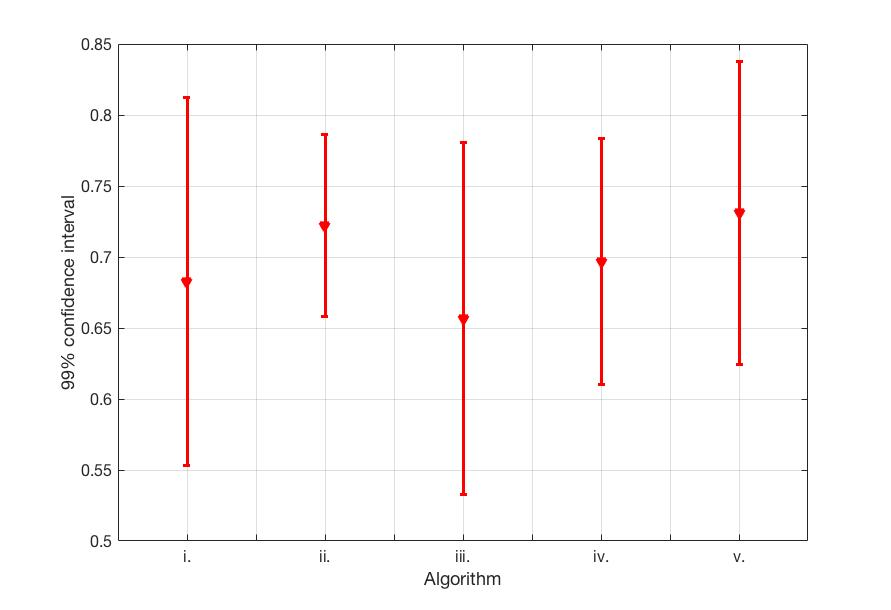
\includegraphics[scale = 0.5]{5.jpg}
According to the 99\% confidence interval we get from t-distribution, the performance of each method is not significantly different from the others. Moreover, the ranking of the first 4 methods is $ii. > iv. > i. > iii.$. However, $v.$ is really hard to compare with others because of the randomization process in it. We could find an average accuracy = 0.731 after adjusting the sampling ratio of training data set to 80\% which is the best of all methods introduced. Thus, roughly speaking, the ranking might be $v. >ii. > iv. > i. > iii.$  
